%-------------------------------------------------------------------------------
%   PACKAGES AND THEMES
%-------------------------------------------------------------------------------

\documentclass[10pt]{beamer}

\mode<presentation> {

    \usetheme{default} %%%
    %\usetheme{Antibes} %%%
    %\usetheme{Berlin} %%%
    %\usetheme{Hannover} %%%
    %\usetheme{Luebeck} %%%
    %\usetheme{Malmoe} %%%
    %\usetheme{Pittsburgh} %%
    %\usetheme{Rochester} %%%
    %\usetheme{Singapore} %%%
    %\usetheme{Szeged} %%%

    %\usecolortheme{beaver}
    %\usecolortheme{beetle}
    %\usecolortheme{crane}
    %\usecolortheme{dolphin}
    %\usecolortheme{dove}
    %\usecolortheme{fly}
    %\usecolortheme{lily}
    %\usecolortheme{orchid}
    \usecolortheme{rose}
    %\usecolortheme{seagull}
    %\usecolortheme{seahorse}
    %\usecolortheme{whale}

    \usefonttheme[onlymath]{serif}

    % Remove the footer line in all slides
    %\setbeamertemplate{footline}

    % Replace the footer line in all slides with a simple slide count
    \setbeamertemplate{footline}[page number]

    % Remove the navigation symbols from the bottom of all slides
    \setbeamertemplate{navigation symbols}{}
}

\usepackage{fontspec}
\setsansfont{Liberation Sans}
\setmainfont{Liberation Serif}
\setmonofont[Scale=0.9]{Hack}

\usepackage{graphicx} % Required for including pictures
\usepackage{wrapfig} % Allows in-line images such as the example fish picture
\usepackage[english]{babel} % Language hyphenation and typographical rules
\usepackage{hyperref}
\hypersetup{
    %draft, % Uncomment to remove all links (for printing in black and white)
    colorlinks = true,
    breaklinks = true,
    bookmarks  = true,
    bookmarksnumbered,
}
\usepackage{mathtools}
\usepackage{amsmath}
\usepackage{bookmark}
\bookmarksetup{numbered}
\usepackage{csquotes}
\usepackage{booktabs} % Horizontal rules in tables
\graphicspath{{pic/}} % Specifies the directory where pictures are stored

\usepackage[numbers,sort&compress]{natbib}
\bibliographystyle{acm}

%-------------------------------------------------------------------------------
%   CODE INCLUSION CONFIGURATION
%-------------------------------------------------------------------------------

\usepackage{listings}

\lstset{language=C,
        frame=LR,
        belowcaptionskip=1\baselineskip,
        breaklines=true,
        xleftmargin=\parindent,
        showstringspaces=false,
        basicstyle=\footnotesize\ttfamily,
        keywordstyle=\bfseries\color{Green},
        commentstyle=\color{Gray},
        identifierstyle=\color{black},
        stringstyle=\color{Orange},
        %numbers=left, % Line numbers on left
        %firstnumber=1, % Line numbers start with line 1
        %numberstyle=\scriptsize\ttfamily\color{Brown},
}

%-------------------------------------------------------------------------------
%   TITLE PAGE
%-------------------------------------------------------------------------------

% The short title appears at the bottom of every slide, the full title is only
% on the title page
\title[Bazang: Kernel Level Tracing for Applications]{Bazang: Kernel Level Tracing for Applications}

\author{Kuan-Yen Chou}
\institute[UIUC] {
    University of Illinois at Urbana-Champaign \\ % Institution full name
    \medskip
    \textit{kychou2@illinois.edu} % Your email address
}
\date{\today} % Date, can be changed to a custom date

\begin{document}

\begin{frame}
\titlepage % Print the title page as the first slide
\end{frame}

\begin{frame}
\frametitle{Overview} % Table of contents slide
\begin{NoHyper}
\tableofcontents
\end{NoHyper}
\end{frame}

%-------------------------------------------------------------------------------
%   PRESENTATION SLIDES
%-------------------------------------------------------------------------------

\section{Introduction}

%------------------------------------------------

\subsection{Kernel Level Tracing for Applications}
\begin{frame}
\frametitle{Kernel Level Tracing for Applications}

\end{frame}

\subsection{\texttt{SO\_TIMESTAMPING}: Requesting Timestamps}
\begin{frame}[fragile]
\frametitle{\texttt{SO\_TIMESTAMPING}: Requesting Timestamps}
\begin{itemize}
\item setsockopt(3) - socket-wise configuration
      {\small
      \begin{verbatim}
setsockopt(fd, SOL_SOCKET, SO_TIMESTAMPING,
           (void *)&opt, sizeof(opt))\end{verbatim}
      }
\item cmsg(3) via sendmsg - message-wise configuration (only applies to TX
      timestamps)
      {\small
      \begin{verbatim}
msg->msg_control = cmsg;
msg->msg_controllen = sizeof(cmsg);
sendmsg(fd, msg, 0);\end{verbatim}
      }
\item timestamp options we use
      \begin{itemize}
      \item \small\texttt{SOF\_TIMESTAMPING\_RX\_SOFTWARE}
      \item \small\texttt{SOF\_TIMESTAMPING\_TX\_SCHED}
      \item \small\texttt{SOF\_TIMESTAMPING\_TX\_SOFTWARE}
      \item \small\texttt{SOF\_TIMESTAMPING\_TX\_ACK}
      \item \small\texttt{SOF\_TIMESTAMPING\_SOFTWARE}
      \item \small\texttt{SOF\_TIMESTAMPING\_OPT\_ID}
      \item \small\texttt{SOF\_TIMESTAMPING\_OPT\_TSONLY}
      \end{itemize}
\end{itemize}
\end{frame}

\subsection{\texttt{SO\_TIMESTAMPING}: Receiving Timestamps}
\begin{frame}[fragile]
\frametitle{\texttt{SO\_TIMESTAMPING}: Receiving Timestamps}
    When events occur, timestamps will be generated as the control message.
\begin{block}{\normalsize Receiving TX timestamps (scheduled, sent, acked)}
      TX timestamps will be looped back to system error queue with an empty
      payload. (\small\texttt{SOF\_TIMESTAMPING\_OPT\_TSONLY})
      {\small
      \begin{verbatim}
recvmsg(fd, &msg, MSG_ERRQUEUE);\end{verbatim}
      }
\end{block}
\begin{block}{\normalsize Receiving RX timestamp (received)}
      RX timestamp will be attached to the original packet.
      {\small
      \begin{verbatim}
recvmsg(fd, &msg, 0);\end{verbatim}
      }
\end{block}
\end{frame}

%------------------------------------------------

\section{Integration with RPC frameworks}

%------------------------------------------------

\subsection{Integration with RPC frameworks: rpclib/Asio}
\begin{frame}
\frametitle{Integration with RPC frameworks: rpclib/Asio}
    Changes:
\href{https://github.com/kyechou/rpclib/commit/568cc625ceaff7c3a9579db56b1d3cea513d7f55}{[view
    on GitHub]}
\begin{enumerate}
\item Set up socket options on both server/client sides right after the
      connection is accepted
\item Implement a wrapper function for recv(3) based on recvmsg(3) to receive
      generated timestamps
\item Read from the error queue asynchronously to get TX timestamps.
\end{enumerate}

Moved to gRPC for:
\begin{itemize}
\item Production grade framework, used by Google itself, Netflix, Cisco,
      Juniper, etc.
\item Better structured code base, easier to read, develop, and maintain
\item Mature event-driven model
\item Tracing buffers for collecting timestamps
\item RPC metadata support
\item TX timestamps support
\end{itemize}
\end{frame}

\subsection{Integration with RPC frameworks: gRPC}
\begin{frame}
\frametitle{Integration with RPC frameworks: gRPC}
    Changes:
\href{https://github.com/kyechou/grpc/commit/8fe57c107e0cff374ad4feba9a12231d877f5d31}{[view
    on GitHub]}
\begin{enumerate}
\item Enable support for Linux error queue
\item Additional client/server APIs for enabling and disabling timestamps
\item Set up timestamps reporting options on both sides right after the
      connection is accepted
\item Pass timestamps arguments as RPC metadata for detailed tracing information
\item Reconstruct timestamps arguments from RPC metadata
\item Implement RX timestamp functions
\end{enumerate}
\end{frame}

%------------------------------------------------

\section{Results}

%------------------------------------------------

\subsection{Sample Client/Server with gRPC}
\begin{frame}[fragile]
\frametitle{Sample Client/Server with gRPC}
Simple echo server/client:
\begin{block}{\normalsize server.cc}
      {\small
      \begin{verbatim}
...
server->enable_timestamps(&process_timestamps);
server->Wait();\end{verbatim}
      }
\end{block}
\begin{block}{\normalsize client.cc}
      {\small
      \begin{verbatim}
...
Client client(channel);
channel->enable_timestamps(&process_timestamps);
reply = client.echo(input);\end{verbatim}
      }
\end{block}
\end{frame}

\begin{frame}[fragile]
\frametitle{Sample Client/Server with gRPC}
User-provided callback:
\begin{block}{\normalsize timestamps.cc}
      {\small
      \begin{verbatim}
void process_timestamps(grpc::TimestampsArgs *arg,
                        grpc::Timestamps *timestamps)
{
    // Users can do anything with the timestamps and
    // metadata information
}\end{verbatim}
      }
\end{block}
\end{frame}

\begin{frame}[fragile]
\frametitle{Sample Client/Server with gRPC}
\begin{columns}[c]
\column{.47\textwidth}
\begin{block}{}
      {\scriptsize
      \begin{verbatim}
$ ./client
===========================
UUID:      2786a4f3-3732-4e21-8d7d-...
Name:      echo
Type:      request
Peer:      ipv6:[::1]:50051
Seq No:    561
sendmsg(): 1547162128.244888239
scheduled: 1547162128.244894091
sent:      1547162128.244895179
received:  0.000000000
acked:     1547162128.244900775
===========================
UUID:      2786a4f3-3732-4e21-8d7d-...
Name:      echo
Type:      response
Peer:      ipv6:[::1]:50051
Seq No:    0
sendmsg(): 0.000000000
scheduled: 0.000000000
sent:      0.000000000
received:  1547162128.245135628
acked:     0.000000000\end{verbatim}
      }
\end{block}

\column{.47\textwidth}
\begin{block}{}
      {\scriptsize
      \begin{verbatim}
$ ./server
===========================
UUID:      2786a4f3-3732-4e21-8d7d-...
Name:      echo
Type:      request
Peer:      ipv6:[::1]:41362
Seq No:    0
sendmsg(): 0.000000000
scheduled: 0.000000000
sent:      0.000000000
received:  1547162128.244895572
acked:     0.000000000
===========================
UUID:      2786a4f3-3732-4e21-8d7d-...
Name:      echo
Type:      response
Peer:      ipv6:[::1]:41362
Seq No:    439
sendmsg(): 1547162128.245126207
scheduled: 1547162128.245132689
sent:      1547162128.245135146
received:  0.000000000
acked:     1547162128.245151533\end{verbatim}
      }
\end{block}
\end{columns}
\end{frame}

\subsection{Visualization (using Redash)}
\begin{frame}
\frametitle{Visualization (using Redash)}
Requests:
\begin{figure}
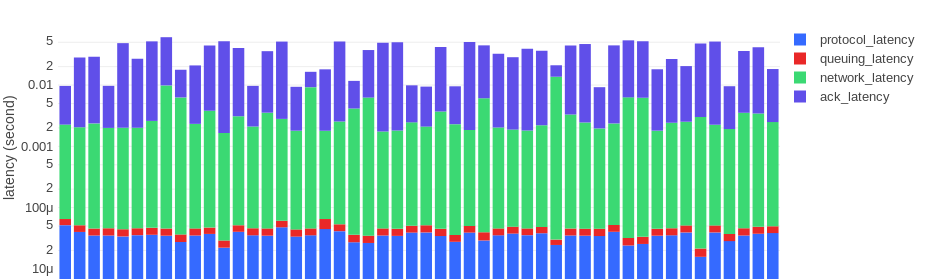
\includegraphics[width=\linewidth]{grpc-requests-latencies}
\end{figure}
Responses:
\begin{figure}
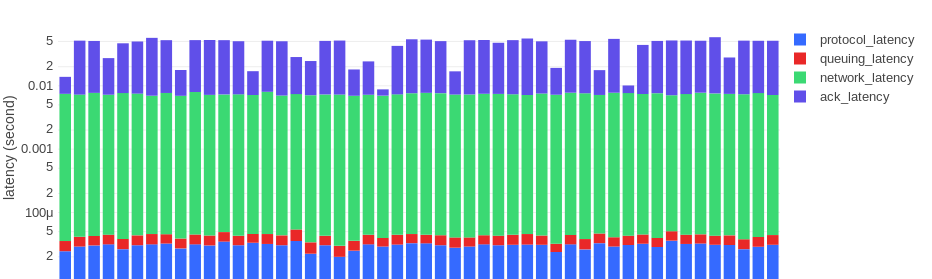
\includegraphics[width=\linewidth]{grpc-responses-latencies}
\end{figure}
\end{frame}

\subsection{Special Case: Network Congestion}
\begin{frame}
\frametitle{Special Case: Network Congestion}
Requests:
\begin{figure}
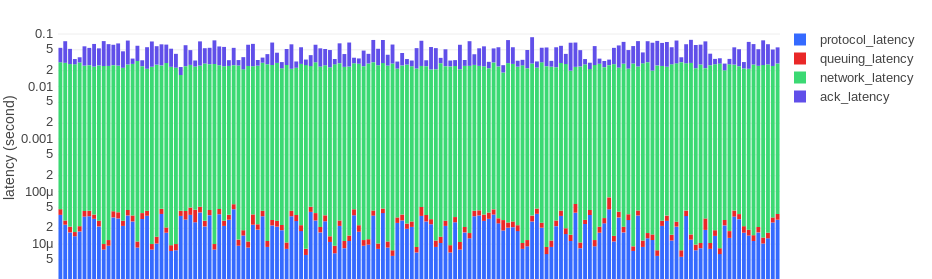
\includegraphics[width=\linewidth]{congested-requests}
\end{figure}
Responses:
\begin{figure}
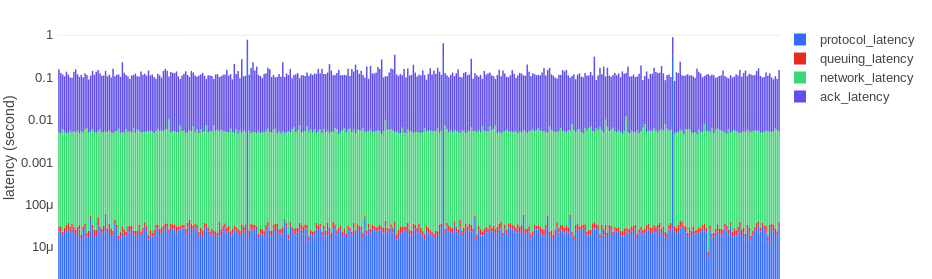
\includegraphics[width=\linewidth]{congested-responses}
\end{figure}
\end{frame}

\subsection{Future Work}
\begin{frame}
\frametitle{Future Work}
\begin{itemize}
\item TensorFlow and Distributed TensorFlow
    \begin{itemize}
        \item Build TensorFlow with this patched gRPC
        \item In order to get the performance bottlenecks of the distributed applications
    \end{itemize}
\item Benchmarking
    \begin{itemize}
        \item Benchmark the patched gRPC to know how much performance overhead caused by enabling the timestamping functions
    \end{itemize}
\end{itemize}
\end{frame}

%------------------------------------------------

%\begin{frame}
%\frametitle{Multiple Columns}
%\begin{columns}[c] % "c": centered vertical alignment, "t": top vertical alignment
%
%\column{.45\textwidth} % Left column and width
%\textbf{Heading}
%\begin{enumerate}
%\item Statement
%\item Explanation
%\item Example
%\end{enumerate}
%
%\column{.5\textwidth} % Right column and width
%Lorem ipsum dolor sit amet, consectetur adipiscing elit. Integer lectus nisl,
%ultricies in feugiat rutrum, porttitor sit amet augue. Aliquam ut tortor mauris.
%Sed volutpat ante purus, quis accumsan dolor.
%
%\end{columns}
%\end{frame}

%------------------------------------------------

%\begin{frame}
%\frametitle{Table}
%\begin{table}
%\begin{tabular}{l l l}
%\toprule
%\textbf{Treatments} & \textbf{Response 1} & \textbf{Response 2}\\
%\midrule
%Treatment 1 & 0.0003262 & 0.562 \\
%Treatment 2 & 0.0015681 & 0.910 \\
%Treatment 3 & 0.0009271 & 0.296 \\
%\bottomrule
%\end{tabular}
%\caption{Table caption}
%\end{table}
%\end{frame}

%------------------------------------------------

%\begin{frame}
%\frametitle{Theorem}
%\begin{theorem}[Mass--energy equivalence]
%$E = mc^2$
%\end{theorem}
%\end{frame}

%------------------------------------------------

%\begin{frame}[fragile] % Needed for verbatim
%\frametitle{Verbatim}
%\begin{example}[Theorem Slide Code]
%\begin{verbatim}
%\begin{frame}
%\frametitle{Theorem}
%\begin{theorem}[Mass--energy equivalence]
%$E = mc^2$
%\end{theorem}
%\end{frame}\end{verbatim}
%\end{example}
%\end{frame}

%------------------------------------------------

%\begin{frame}
%\frametitle{Figure}
%Uncomment the code on this slide to include your own image from the same
%directory as the template .TeX file.
%%\begin{figure}
%%\includegraphics[width=0.8\linewidth]{test}
%%\end{figure}
%\end{frame}

%------------------------------------------------

%\begin{frame}[fragile] % Needed for verbatim
%\frametitle{Citation}
%An example of the \verb|\cite| command to cite within the presentation:\\~
%
%This statement requires citation \cite{figueredo2009}.
%\end{frame}

%------------------------------------------------

%\begin{frame}
%\frametitle{References}
%{\footnotesize
%    \setsansfont{Liberation Serif}
%    \bibliography{ref}
%}
%\end{frame}

%-------------------------------------------------------------------------------

\end{document}
